\documentclass{thesis}
%\usepackage[colorlinks, urlcolor=blue, linkcolor=red, citecolor=red, linktocpage=true]{hyperref}
\usepackage[linktocpage=true]{hyperref}
\usepackage{russianplural}
\usepackage{amsmath}
\usepackage{amssymb}
\usepackage{amsfonts}
\usepackage{totcount}
\usepackage{mdwlist}
\usepackage{makecell}
\usepackage{booktabs}
\usepackage{hyperref}
%\usepackage{showframe}
\usepackage{setspace}
\usepackage{caption}
\usepackage{fixme}
\usepackage{titlesec}
% \usepackage{float}
\usepackage{listings}
\usepackage{algorithm}
\usepackage{listings}
\usepackage{xcolor}
\usepackage{graphicx}%Вставка картинок правильная
\fxsetup{status=draft} % <====== add this line
\usepackage{float}%"Плавающие" картинки

\usepackage{wrapfig}%Обтекание фигур (таблиц, картинок и прочего)
\graphicspath{{noiseimages/}}
\definecolor{codegreen}{rgb}{0,0.6,0}
\definecolor{codegray}{rgb}{0.5,0.5,0.5}
\definecolor{codepurple}{rgb}{0.58,0,0.82}
\definecolor{backcolour}{rgb}{0.95,0.95,0.92}

\lstdefinestyle{mystyle}{
    backgroundcolor=\color{backcolour},   
    commentstyle=\color{codegreen},
    keywordstyle=\color{magenta},
    numberstyle=\tiny\color{codegray},
    stringstyle=\color{codepurple},
    basicstyle=\ttfamily\footnotesize,
    breakatwhitespace=false,         
    breaklines=true,                 
    captionpos=b,                    
    keepspaces=true,                 
    numbers=left,                    
    numbersep=5pt,                  
    showspaces=false,                
    showstringspaces=false,
    showtabs=false,                  
    tabsize=2
}

\lstset{style=mystyle}

\usepackage[noend]{algpseudocode}
\newcommand{\head}[1]{\textnormal{\textbf{#1}}}

\DeclareMathOperator*{\argmax}{arg\,max}

\makeatletter
\newbox\sf@box
\newenvironment{SubFloat}[2][]%
{\def\sf@one{#1}%
	\def\sf@two{#2}%
	\setbox\sf@box\hbox
	\bgroup}%
{ \egroup
	\ifx\@empty\sf@two\@empty\relax
	\def\sf@two{\@empty}
	\fi
	\ifx\@empty\sf@one\@empty\relax
	\subfloat[\sf@two]{\box\sf@box}%
	\else
	\subfloat[\sf@one][\sf@two]{\box\sf@box}%
	\fi}
\makeatother

% \usepackage{showframe}

\newtotcounter{bibitems}
\setcounter{bibitems}{0}

\captionsetup[subfloat]{farskip=0pt}
% \setlength{\farskip}{0pt}
% \setlength{\textfloatsep}{18pt}

% \setlength{\intextsep}{0pt}

% \setlength{\belowcaptionskip}{-0.5em}

\graphicspath{{pic/}, {pseudocode/}}
\titlespacing{\paragraph}{1.25cm}{1.5em plus .1ex minus .2ex}{1em}
\captionsetup[table]{skip=-0.4em}
\captionsetup[lstlisting]{font={small}}

\begin{document} % ------------------------------------------------------------
\sloppy

\newpage
\thispagestyle{empty}
\begin{adjustwidth}[]{0cm}{0cm}
\begin{center}
\begin{linespread}{1}


\small{
МИНИСТЕРСТВО ОБРАЗОВАНИЯ И НАУКИ РОССИЙСКОЙ ФЕДЕРАЦИИ\\
Федеральное государственное бюджетное образовательное учреждение\\
высшего образования\\
\textbf{<<Южно-Уральский государственный университет\\
(национальный исследовательский университет)>>\\
Высшая школа электроники и компьютерных наук\\
Кафедра системного программирования}
}


%{\small МИНИСТЕРСТВО ОБРАЗОВАНИЯ И НАУКИ РОССИЙСКОЙ ФЕДЕРАЦИИ\\
%Федеральное государственное бюджетное образовательное учреждение\\
%высшего образования\\}
%\textbf{<<Южно-Уральский государственный университет\\
%(национальный исследовательский университет)>>\\}
%{\small \textbf{Высшая школа электроники и компьютерных наук\\	Кафедра системного программирования\\}}

\vspace{\stretch{1}}

%\parbox[t]{7cm}{
%РАБОТА ПРОВЕРЕНА\\[0.5em]
%Рецензент \\
%Зам. директора по инф.\\ 
%технологиям и безопасности
%\\ ГБУЗ ``ЧОМИАЦ''\\[0.5em]
%\underline{\hspace{2.5cm}} А.С.~Староверов \\[0.5em]
%``\underline{\qquad}''\underline{\hspace{2.5cm}} 2018~г.
%}
%\hfill{}
%\parbox[t]{6.7cm}{
%ДОПУСТИТЬ К ЗАЩИТЕ \\[0.5em]
%Заведующий кафедрой,\\д.ф.-м.н., профессор\\[0.5em]
%{\hspace{2.5cm}} Л.Б.~Соколинский \\[0.5em]
%``\underline{\qquad}''\underline{\hspace{2.5cm}} 2018~г.
%}


%\vspace{\stretch{1}}



\vspace{\stretch{1}}

{
\large\textbf{Разработка системы}

\vspace{-5pt}

\large\textbf{для классификации проектов GitHub}

\vspace{-5pt}

\large\textbf{по популярности}

}
\vspace{2em}

КУРСОВАЯ РАБОТА \\
по дисциплине <<Программная инженерия>>\\
ЮУрГУ -- 09.03.04.2024.308-066.КР


\vspace{\stretch{1}}

\parbox[t]{7cm}{
Нормоконтролер,\\[0.5em]
доктор физ.-мат. наук \\[0.5em]
\underfield{} М.Л.~Цымблер \\[0.5em]
<<\underline{\qquad}>>\underfield{} 2024~г.
}
\hfill{}
\parbox[t]{7cm}{
Научный руководитель \\
доктор физ.-мат. наук\\[0.5em]
\underfield{} М.Л.~Цымблер \\[2.5em]
Автор работы, \\
студент группы КЭ-303\\[0.5em]
\underfield{} Д.И.~Гольденберг \\[2.5em]
Работа защищена с оценкой \\[0.5em]
\underfield{}  \\[0.5em]
<<\underline{\qquad}>>\underfield{} 2024~г.

}

\vspace{\stretch{1}}

Челябинск-2024

\end{linespread}
\end{center}
\end{adjustwidth}

\pagebreak
 % титульный лист

% \thispagestyle{empty}
\setcounter{page}{2}
\newpage
\thispagestyle{empty}

\begin{adjustwidth}{-1.5cm}{0.5cm}
\begin{linespread}{1}
\begin{center}


\small{
МИНИСТЕРСТВО ОБРАЗОВАНИЯ И НАУКИ РОССИЙСКОЙ ФЕДЕРАЦИИ\\
Федеральное государственное бюджетное образовательное учреждение\\
высшего образования\\
\textbf{<<Южно-Уральский государственный университет\\
(национальный исследовательский университет)>>\\
Высшая школа электроники и компьютерных наук\\
Кафедра системного программирования}
}



\vspace{2em}

\hfill{}
\parbox{7cm}{
УТВЕРЖДАЮ \\
Зав. кафедрой СП \\[0.5em]
\underfield{} Л.Б.~Соколинский \\[0.5em]
06.02.2024
}

\vspace{2em}

\textbf{ЗАДАНИЕ} \\
% \parbox[t]{14cm}{
\textbf{на выполнение выпускной квалификационной работы бакалавра}\\
студентке группы КЭ-303\\
Гольденберг Дарье Игоревне,\\
обучающейся по направлению 09.03.04 <<Программная инженерия>> 
% }

\end{center}

\vspace{2em}

{
\small
\begin{enumerate}
	\bf\item Тема работы \rm \\
	Разработка системы для классификации проектов GitHub по популярности.
	\bf\item Срок сдачи студентом законченной работы: \rm
	05.06.2024.

	\bf\item Исходные данные к работе\rm
	\begin{enumerate}%[leftmargin=0.35cm]
		\raggedright
		\item Milovidov A., 2020. Everything You Ever Wanted To Know About GitHub (But Were Afraid To Ask). [Электронный ресурс] URL: https://ghe.clickhouse.tech/
        \item Документация по использованию библиотеки Scikit learn. [Электронный ресурс] URL: https://scikit-learn.org/stable/user\_guide.html 
        \item Soll M., Vosgerau M. ClassifyHub: An Algorithm to Classify GitHub Repositories. [Электронный ресурс] URL: https://doi.org/10.1007/978-3-319-67190-1\_34
	\end{enumerate}

	\bf\item Перечень подлежащих разработке вопросов\rm
	\begin{enumerate}
		
    \item Выполнить анализ предметной области и провести обзор существующих решений.

    \item Выбрать репрезентативный набор признаков и подготовить данные по существующим репозиториям GitHub.

   \item Исследовать различные модели машинного обучения и выбрать наиболее эффективные.

    \item Разработать приложение, которое будет классифицировать проекты по нескольким уровням на основе выбранной модели.
	\end{enumerate}

	\bf\item Дата выдачи задания: \rm
	09.02.2024.
\end{enumerate}

\vspace{1em}

\noindent
\textbf{Научный руководитель}
\hfill
\hbox to 8em{М.Л.~Цымблер\hfill}

\vspace{1em}

\noindent
\textbf{Задание принял к исполнению}
\hfill
\hbox to 8em{Д.И.~Гольденберг\hfill}

}

\thispagestyle{empty}

\end{linespread}
\end{adjustwidth}

\pagebreak


\newpage
%{\linespread{1.1}
\tableofcontents % оглавление
%}

    \newpage
\sectionnonumber{Введение}
\subsection*{Актуальность темы}
Актуальность работы заключается в том, что с развитием технологий тяжело понять, насколько может быть популярен проект, такая система может быть полезна для дальнейшей работы с репозиторием. 

\subsection*{Цель и задачи исследования}
Целью данной работы является разработка системы прогноза популярности проектов GitHub. В качестве исходных данных используются датасет ClickHouse о репозиториях на GitHub. Для достижения поставленной цели необходимо было решить следующие \textit{задачи}:
\begin{enumerateparen}
	\item провести анализ предметной области и обзор научной литературы по тематике исследования;
	\item разработать алгоритм обработки данных;
	\item 
\end{enumerateparen}
\vspace{0.5em}
\subsection*{Структура и объем работы}

Курсовая работа состоит из введения, пяти разделов, заключения и списка литературы. Объем работы составляет n страниц, объем библиографического списка составляет – k наименований.

\subsection*{Содержание работы}

\textbf{Первый раздел, «Обзор работ по тематике исследования»}, содержит обзор на работы по тематике исследования.

\textbf{Второй раздел, «Анализ предметной области»}, описывает постановку задачи и описание данных, которые будут использоваться для анализа.

\textbf{Третий раздел, «Проектирование»}, определяет требования к системе, описаны модели данных и структура приложения.

\textbf{Четвертый раздел, «Реализация»}, описывает реализацию компонентов системы.

\textbf{Пятый раздел, «Тестирование»}, описывает функциональное тестирование работы и эксперименты с разработанными моделями данных.

\textbf{В заключении} приведены основные итоги проделанной работы.
\newpage
\section{Обзор работ по тематике исследования}
\label{subsec:Rewiev}
Исследования, связанные с анализом данных, возникающих при использовании GitHub и разработке продуктов на этой платформе, представляют собой популярную тему для научных исследований.

Так, авторы статьи~\cite{abs-2308-14211} обсуждают проблему классификации отзывов о приложениях, которые содержат важную информацию о потребностях пользователей. Исследователи предлагают подход для создания более обобщенной модели, используя информацию из системы отслеживания задач GitHub, которая содержит ценные данные о потребностях пользователей. После проведения экспериментов, они показывают, что использование размеченных задач из GitHub может улучшить точность и полноту классификации отзывов, особенно для отчетов о багах и запросов на новые функции. В другой статье~\cite{RoccoRSNR23} поднимается важность репозиториев программного обеспечения для управления проектами, включая исходный код, документацию и отчеты об ошибках. Особое внимание уделяется платформе GitHub, которая для помощи разработчикам в поиске подходящих артефактов использует темы (topics), являющимися короткими текстами, присваиваемыми хранимым артефактам. Однако неправильное присвоение тем может негативно сказаться на популярности репозитория. 

Закария Альшара и другие авторы в своей статье~\cite{AlsharaSSS23} рассматривают проблему управления задачами (issues) на платформе GitHub, особенно в случае быстрого роста числа создаваемых задач. Для помощи разработчикам в обработке задач существуют внешние участники, которые исправляют задачи, создавая pull-запросы (Pull Requests, они же PR). Однако часто такие PR не связываются с соответствующими задачами (issues), что затрудняет управление проектом. В статье предлагается использование моделей машинного обучения (ML) для автоматического восстановления связей между PR и задачами на GitHub. Установление связей между PR и задачами ценно, так как это помогает улучшить управление разработкой и обслуживанием проектов, что влияет на популярность и развитие проекта в дальнейшем.

В исследовании~\cite{RamasamySBB23} исследует, как проводится кодирование в области науки о данных на GitHub. Авторы анализируют, как данные ученые переходят между разными этапами работы с данными. Результаты исследования показывают, что кодирование имеет определенные паттерны. Кроме того, авторы попытались обучить модели машинного обучения для предсказания этапов работы с данными и достигли точности примерно 71\%.

О популярных проектах говорят в статье Джесси Айала и ее коллеги~\cite{AyalaG23}, а именно о важности использования непрерывной интеграции и поставки (CI/CD) и политики безопасности в известных и пользующихся интересом проектах с открытым исходным кодом, особенно на GitHub. Исследование показало, что многие проекты не активно используют эти возможности, и призывает управляющих таких проектов уделить им больше внимания для предотвращения уязвимостей. А в другом исследовании~\cite{PuhlfurssMM22} фокусируются на том, как документируется информация о функциональных возможностях программного обеспечения в проектах на GitHub и связана ли она с исходным кодом. Авторы провели анализ 25 популярных репозиториев на GitHub и обнаружили, что хотя документация о функциональности часто присутствует в различных текстовых файлах, она часто неструктурированна, и связь с исходным кодом редко устанавливается, что может привести к затруднениям в его поддержке на долгосрочной перспективе. 

Кроме того, существует статья~\cite{CasalnuovoSRR17}, рассматривающая инструмент GitcProc, который предназначен для анализа проектов на GitHub. Этот инструмент позволяет извлекать информацию о разработке, включая исходный код и историю исправления ошибок. GitcProc может отслеживать изменения в исходном коде и связывать их с функциями с минимальными настройками. Он успешно работает с проектами на разных языках программирования, обнаруживая исправления ошибок и контекст изменений в коде. Помимо этого, стоит также рассмотреть следующую работу~\cite{SollV17}, где авторы обсуждают задачу классификации репозиториев на GitHub, которая представляет собой сложную задачу. Они представляют алгоритм ClassifyHub, основанный на методах ансамблирования, разработанный для соревнования InformatiCup 2017. Этот алгоритм успешно решает задачу классификации с высокой точностью и полнотой, что может быть полезно для различных приложений, таких как рекомендательные системы.

Самой приближенной к поставленной задаче статьей является <<A Cross-Repository Model for Predicting Popularity in GitHub>>~\cite{abs-1902-05216}, в которой рассматривается создание модели для прогнозирования популярности репозиториев на GitHub, используя данные из разных репозиториев. Модель, основанная на рекуррентной нейронной сети LSTM, позволяет более точно предсказывать популярность, чем стандартные методы прогнозирования временных рядов на основе данных из одного репозитория. 

Кроме неё, есть также исследование~\cite{HanDXWY19}, в котором предлагают метод для прогнозирования популярности проектов на GitHub. Он использует 35 признаков, извлеченных из GitHub и Stack Overflow, чтобы классифицировать проекты как популярные или нет. Модель, основанная на случайном лесе, достигает высокой точности значительно превосходит существующие методы. Основными признаками для определения популярности оказались количество веток, количество открытых задач и количество участников проекта.
\newpage
\section{Анализ предметной области}
\label{sec:Background}
\subsection{Описание предметной области}
\label{subsec:Description}

Сайты для хостинга открытого исходного кода, такие как GitHub, например, GitLab, Bitbucket и др, представляют собой цифровые площадки, где разработчики могут хранить, управлять и совместно работать над своими проектами с открытым доступом к исходному коду.

Одной из основных причин популярности таких платформ является идеология открытого исходного кода. Распространение проектов с открытым исходным кодом способствует коллективному развитию программного обеспечения, позволяя разработчикам из разных уголков мира вносить свой вклад, исправлять ошибки и улучшать функционал. Это приводит к созданию более качественного, надежного и инновационного программного обеспечения.

Сами сайты основаны на системах контроля версий, которые являются ключевым инструментом в разработке программного обеспечения, обеспечивая эффективное управление изменениями в исходном коде проекта. Они позволяют разработчикам отслеживать и сохранять историю изменений в коде, а также управлять конфликтами и совмещать работу множества разработчиков. Согласно рейтингу Tagline~\cite{SCVRating} самой популярной системой контроля версий считается Git, что представлено на рисунке~\ref{ris:scvrating}.

\begin{figure}[h]
    \centering
    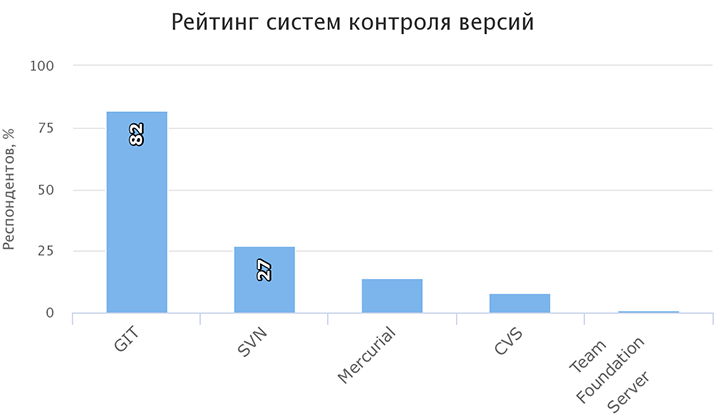
\includegraphics[width=0.9\linewidth]{pic/scvrating.png}
    \caption{Рейтинг систем контроля версий}
    \label{ris:scvrating}
\end{figure}
\vspace{1em}

Git, созданный Линусом Торвальдсом в 2005 году, стал стандартом для управления исходным кодом в различных проектах, от небольших локальных до масштабных проектов с открытым исходным кодом, таких как ядро Linux и сам GitHub.

GitHub -- это веб-платформа для хранения и совместной разработки проектов с открытым исходным кодом. С момента своего запуска в 2008 году GitHub стал одной из самых популярных и важных платформ для разработчиков по всему миру. Его привлекательность обусловлена множеством факторов. Так, издание The New Stack~\cite{GitRating} собрало статистику по используемым хостингам кода на основе Git за 2018-2019 года (рис.~\ref{ris:gitrating}). Несмотря на падение популярности GitHub в 2019 году по сравнению с 2018, он всё ещё остается самым используемым сайтом для расположения своего кода в рамках репозиториев.

\begin{figure}[h]
    \centering
    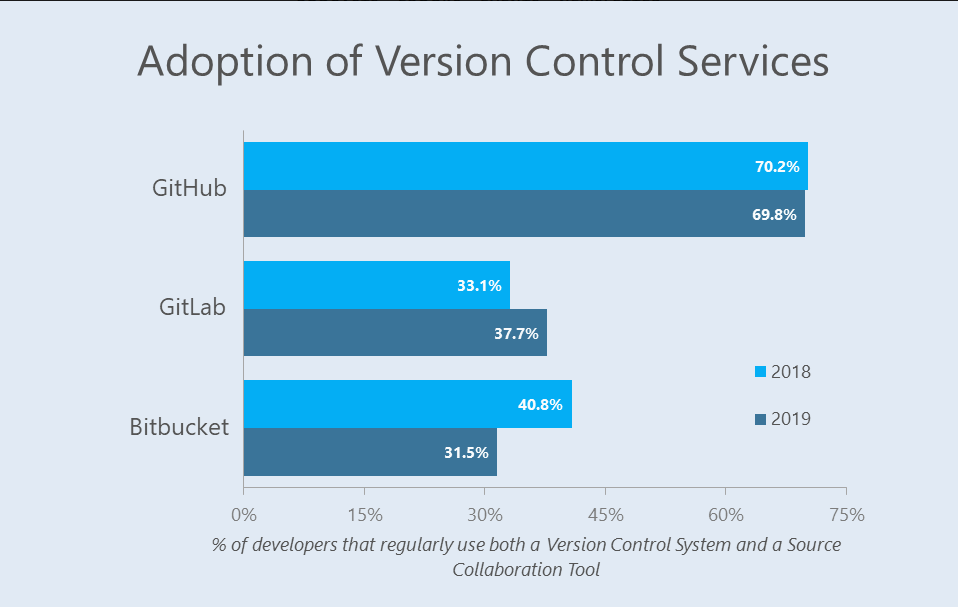
\includegraphics[width=1\linewidth]{pic/gitrating.png}
    \vspace{-1em}\caption{Рейтинг хостингов кода на основе Git}
    \label{ris:gitrating}
\end{figure}
\vspace{1em}

Каждый проект на GitHub представлен в виде репозитория, где хранятся файлы проекта и история их изменений. Для отслеживания действий других пользователей с текущим репозиторием на GitHub используются различные параметры.

\begin{itemizecustom}
    \item Звезды (Stars): Звезды представляют собой показатель популярности проекта. Пользователи GitHub могут добавлять звезды к проектам, которые им нравятся или которые они хотят отслеживать. Чем больше звезд у проекта, тем он популярнее.

    \item Форки (Forks): Форки представляют собой копии репозитория проекта, созданные другими пользователями. Форк может использоваться для внесения изменений в проект без изменения оригинального кода. Чем больше форков у проекта, тем больше разработчиков заинтересовано в его доработке и участии.

    \item Проблемы (Issues): Проблемы представляют собой список задач, багов или идей для улучшения проекта. Количество проблем может служить показателем активности и вовлеченности сообщества в развитие проекта.

    \item Запросы на слияние (Pull Requests): Запросы на слияние представляют собой предложения от разработчиков о внесении изменений в код проекта. Они могут быть использованы для исправления ошибок, добавления нового функционала или внесения других улучшений.
\end{itemizecustom}

Все эти метрики помогают разработчикам оценивать популярность и активность проектов на GitHub. Звезды и форки позволяют судить о популярности проекта среди пользователей, а проблемы и запросы на слияние -- об активности и вовлеченности сообщества разработчиков.

Использование GitHub и его метрик стало стандартной практикой в сообществе разработчиков благодаря его открытости, удобству использования и широким возможностям для совместной работы и обмена знаниями.

\subsection{Обзор аналогов и существующих решений}
\label{subsec:Analogues}

Исследования, посвященные анализу данных, связанных с использованием платформы GitHub и разработкой программного обеспечения на этой платформе, являются актуальной и распространенной темой для научных исследований.

Так, авторы статьи~\cite{abs-2308-14211} обсуждают проблему классификации отзывов о приложениях, которые содержат важную информацию о потребностях пользователей. Исследователи предлагают подход для создания более обобщенной модели, используя информацию из системы отслеживания задач GitHub, которая содержит ценные данные о потребностях пользователей. После проведения экспериментов, они показывают, что использование размеченных задач из GitHub может улучшить точность и полноту классификации отзывов, особенно для отчетов о багах и запросов на новые функции. 

В работе~\cite{RoccoRSNR23} поднимается важность репозиториев программного обеспечения для управления проектами, включая исходный код, документацию и отчеты об ошибках. Особое внимание уделяется платформе GitHub, которая для помощи разработчикам в поиске подходящих артефактов использует темы (topics), являющимися короткими текстами, присваиваемыми хранимым артефактам. Однако неправильное присвоение тем может негативно сказаться на популярности репозитория. 

Закария Альшара и другие авторы в своей статье~\cite{AlsharaSSS23} рассматривают проблему управления задачами (issues) на платформе GitHub, особенно в случае быстрого роста числа создаваемых задач. Для помощи разработчикам в обработке задач существуют внешние участники, которые исправляют задачи, создавая pull-запросы (Pull Requests, они же PR). Однако часто такие PR не связываются с соответствующими задачами (issues), что затрудняет управление проектом. В статье предлагается использование моделей машинного обучения (ML) для автоматического восстановления связей между PR и задачами на GitHub. Установление связей между PR и задачами ценно, так как это помогает улучшить управление разработкой и обслуживанием проектов, что влияет на популярность и развитие проекта в дальнейшем.

В работе~\cite{RamasamySBB23} исследует, как проводится кодирование в области науки о данных на GitHub. Авторы анализируют, как данные ученые переходят между разными этапами работы с данными. Результаты исследования показывают, что кодирование имеет определенные паттерны. Кроме того, авторы попытались обучить модели машинного обучения для предсказания этапов работы с данными и достигли точности примерно 71\%.

О популярных проектах говорят в статье Джесси Айала и ее коллеги~\cite{AyalaG23}, а именно о важности использования непрерывной интеграции и поставки (CI/CD) и политики безопасности в известных и пользующихся интересом проектах с открытым исходным кодом, особенно на GitHub. Исследование показало, что многие проекты не активно используют эти возможности, и призывает управляющих таких проектов уделить им больше внимания для предотвращения уязвимостей. 

Кроме того, в исследовании~\cite{PuhlfurssMM22} фокусируются на том, как документируется информация о функциональных возможностях программного обеспечения в проектах на GitHub и связана ли она с исходным кодом. Авторы провели анализ 25 популярных репозиториев на GitHub и обнаружили, что хотя документация о функциональности часто присутствует в различных текстовых файлах, она часто неструктурированна, и связь с исходным кодом редко устанавливается, что может привести к затруднениям в его поддержке на долгосрочной перспективе. 

Статья~\cite{CasalnuovoSRR17} рассматривает инструмент GitcProc, который предназначен для анализа проектов на GitHub. Этот инструмент позволяет извлекать информацию о разработке, включая исходный код и историю исправления ошибок. GitcProc может отслеживать изменения в исходном коде и связывать их с функциями с минимальными настройками. Он успешно работает с проектами на разных языках программирования, обнаруживая исправления ошибок и контекст изменений в коде. 

Помимо этого, стоит также рассмотреть работу~\cite{SollV17}, где авторы обсуждают задачу классификации репозиториев на GitHub, которая представляет собой сложную задачу. Они представляют алгоритм ClassifyHub, основанный на методах ансамблирования, разработанный для соревнования InformatiCup 2017. Этот алгоритм успешно решает задачу классификации с высокой точностью и полнотой, что может быть полезно для различных приложений, таких как рекомендательные системы.

Самой приближенной к поставленной задаче статьей является <<A Cross-Repository Model for Predicting Popularity in GitHub>>~\cite{abs-1902-05216}, в которой рассматривается создание модели для прогнозирования популярности репозиториев на GitHub, используя данные из разных репозиториев. Модель, основанная на рекуррентной нейронной сети LSTM, позволяет более точно предсказывать популярность, чем стандартные методы прогнозирования временных рядов на основе данных из одного репозитория. 

Кроме неё, есть также исследование~\cite{HanDXWY19}, в котором предлагают метод для прогнозирования популярности проектов на GitHub. Он использует 35 признаков, извлеченных из GitHub и Stack Overflow, чтобы классифицировать проекты как популярные или нет. Основными признаками для определения популярности оказались количество веток, количество открытых задач и количество участников проекта.

\subsection{Теоретический базис}
\label{sec:Models}

В этом разделе рассматриваются основные концепции и методы машинного обучения, которые лежат в основе разработки моделей для классификации и регрессии. Машинное обучение -- это раздел искусственного интеллекта, который изучает методы анализа данных и построения предсказательных моделей без явного программирования. Одним из ключевых направлений в машинном обучении является обучение с учителем, где модели создаются на основе предварительно размеченных данных.~\cite{books_daglib_0033642} Чаще встречаются модели двух типов: модель классификации и модель регрессии.

\textit{Модели классификации} являются методами обучения с учителем, цель которых заключается в том, чтобы прогнозировать принадлежность объекта к одной из заданных категорий или классов на основе набора предварительно размеченных данных. Модели классификации используют алгоритмы, которые находят закономерности в данных и создают функцию, относящую новый объект к одному из заранее определенных классов.

Рассмотрим модели, которые будут использованы для работы.

\textbf{Decision Tree (Дерево решений)}
    
Дерево решений строит структуру в виде дерева, в которой каждый узел представляет собой тест на значение определенного признака, а каждое ребро - результат этого теста.~\cite{izza2020explaining} Для построения дерева используются различные алгоритмы, например, алгоритм CART (классификация и регрессия на основе дерева). Процесс построения дерева продолжается, пока не будет выполнен какой-то критерий останова, например, достигнута максимальная глубина дерева или узел содержит объекты только одного класса.

\textbf{Random Forest (Случайный лес)}

Random Forest строит ансамбль деревьев решений, каждое из которых обучается на случайной подвыборке данных.~\cite{breiman2001random} В процессе построения дерева для каждого разбиения выбирается случайный поднабор признаков. После построения всех деревьев в ансамбле, предсказание производится путем агрегации результатов всех деревьев, например, путем голосования (в случае классификации) или усреднения (в случае регрессии).

\textbf{Gradient Boosting (Градиентный бустинг)} 

Gradient Boosting последовательно обучает слабые модели, каждая из которых предсказывает остатки (разницу между истинными значениями и предсказанными значениями) предыдущей модели.~\cite{hastie2001elements} На каждом шаге минимизируется функция потерь (например, среднеквадратичная ошибка для задачи регрессии) с помощью градиентного спуска. Таким образом, каждая новая модель исправляет ошибки предыдущей модели.

\textbf{AdaBoost}
    
AdaBoost обучает слабые модели на последовательно изменяющихся весах обучающих образцов.~\cite{Hastie2009MulticlassA} На каждой итерации модель фокусируется на объектах, которые были классифицированы неправильно на предыдущих итерациях. После обучения всех моделей, их прогнозы комбинируются с помощью взвешенного голосования.

\textbf{Gaussian Naive Bayes (Наивный байесовский классификатор)}

Этот классификатор основан на применении теоремы Байеса с допущением о независимости между признаками.~\cite{Zhang2004} Он предполагает, что каждый признак влияет на класс независимо от других признаков. При классификации модель оценивает вероятность принадлежности объекта к каждому классу и выбирает класс с наибольшей вероятностью.

\textit{Модели регрессии} также являются методами обучения с учителем, но в отличие от классификации, их цель состоит в прогнозировании непрерывных значений целевой переменной на основе имеющихся данных. Модели регрессии стремятся к поиску математической функции, которая наилучшим образом описывает связь между входными признаками и выходными значениями.

\textbf{Linear Regression (Линейная регрессия) }

Линейная регрессия моделирует линейную зависимость между предикторами и целевой переменной. Она находит коэффициенты линейной функции таким образом, чтобы минимизировать сумму квадратов разностей между наблюдаемыми и предсказанными значениями.

Для моделей регрессии Decision Tree, Random Forest, Gradient Boosting главное отличие от их использования в классификации заключается в том, как они строят свои прогнозы и как оценивают качество модели.~\cite{Nunez2011} Так, Случайный лес после обучения всех деревьев результаты агрегируются, например, путем усреднения, чтобы получить окончательный прогноз, а для регрессионных Деревьев решений обычно используется критерий ветвления, такой как среднеквадратичная ошибка.

% Formatting of listings
\lstset{language=C, frame=L, basicstyle=\footnotesize,%\sffamily,
	keywordstyle=\bfseries, showstringspaces=false, xleftmargin=\parindent, numbers=none, numberstyle=\tiny, stepnumber=2, numbersep=12pt}
\newpage
\section{Проектирование}
\label{sec:Design}

В разделе 3.1. представлены функциональные и нефункциональные требования к системе. В разделе 3.2. описывается обработка данных. В разделе 3.3. представлено описание прогнозных моделей. В разделе 3.4. представлен описан модуль прогнозирования.

\subsection{Требования к системе}

Перечисление требований в зависимости от дальнейших выбранных библиотек и интеграций.

\subsection{Обработка данных}

Для дальнейшей работы с данными их необходимо получить из представленного датасета.

\subsection{Прогнозные модели}

Для более точного и достоверного результата необходимо правильно сформировать модели для дальнейшего анализа.

\subsection{Модуль прогнозирования}

Выбор наиболее подходящего алгоритма для прогнозирования в зависимости от приоритетной потребности.

\newpage
\section{Реализация}
\label{sec:Realization}

Тут какой-то текст про то, что в каких разделах реализовано.

\subsection{Обработка данных для модели}
\label{subsec:Parser}

В силу того, что данные из датасета ClickHouse было решено получать из веб-приложения, необходимо разработать способ, которым можно корректно их преобразовать.

Для этой цели был разработан класс, содержащий несколько методов. Самый важный метод позволяет извлекать данные из разметки страны формата html. Этот метод принимает параметр, который определяет желаемый объем данных для извлечения. 

Данная функция имитирует взаимодействие с веб-страницей, используя библиотеку Selenium WebDriver для управления браузером. Он создает виртуальное окружение браузера, отправляет запрос. После ожидания получения результата в течение 10 секунд данные извлекаются из таблицы на веб-странице с использованием библиотеки Beautiful Soup, предназначенной для анализа HTML-файлов. 

Полученные данные могут быть представлены в различных форматах, таких как JSON, CSV и другие. Для работы в дальнейшем будет использоваться формат CSV для обработки. Так, было получено около трехсот тысяч данных с учетом того, что действия в рамках проекта на платформе GitHub выполнялись последние 8 лет.

\subsection{Обучение модели}
\label{subsec:Learning}

Для решения задачи классификации на основе данных платформы GitHub был разработан класс GitHubClassifier. Этот класс содержит несколько методов, предназначенных для обработки данных, обучения моделей и оценки их производительности.

Класс инициализируется путем загрузки данных из CSV-файла и предварительной обработки. Данные подвергаются масштабированию с использованием метода MinMaxScaler из библиотеки sklearn.preprocessing, что позволяет привести значения признаков к одному масштабу.

Для обучения моделей классификации, таких как RandomForestClassifier и GradientBoostingClassifier из библиотеки sklearn.ensemble, используются подготовленные данные. Обученные модели позволяют прогнозировать классы новых данных и оценивать их точность с помощью методов count\_f1, count\_precision и count\_recall, возвращающих значения F1-меры, точности и полноты соответственно.

Также предоставлены методы для вывода матрицы ошибок (get\_confusion\_matrix) в форме графика (plot\_confusion\_matrix), сохранения и загрузки обученных моделей (save\_model и load\_model). Эти методы обеспечивают анализ результатов классификации и позволяют использовать обученные модели для прогнозирования классов новых данных.

\subsection{Графический интерфейс (веб-страница)}
\label{subsec:gui}

В качестве первичного графического интерфейса и возможности отображения работы с моделью было выбрано веб-приложение, которое написано на популярном фреймворке Flask. 

На главной странице отображается форма (рис.~\ref{ris:form-data}) для добавления параметров репозитория, что необходимы для определения модели ранга популярности. 

\begin{center}
    \begin{figure}[H]
        \center{\includegraphics[width=0.4\linewidth]{image}}
        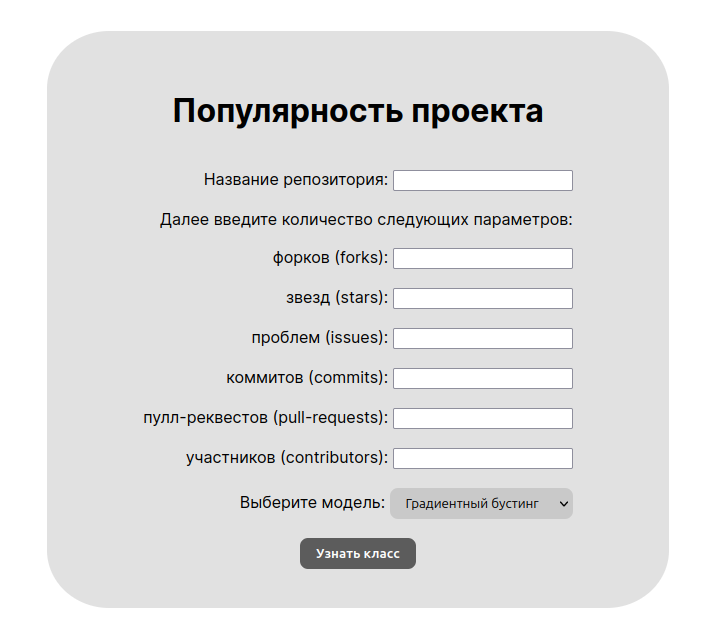
\includegraphics[scale=0.5]{pic/form-data.png}
        \caption{Форма для ввода данных}
        \label{ris:form-data}
    \end{figure}
\end{center}
\vspace{1.5em}

Кроме того, можно выбрать модель, на базе которой будет определен класс популярности проекта. После получения данные проходят обработку, и открывается страницу, на которой отображен результат определения полученного ранга с перечислением того, какие данные были отправлены (рис.~\ref{ris:result-data})

\begin{center}
    \begin{figure}[H]
        \center{\includegraphics[width=0.4\linewidth]{image}}
        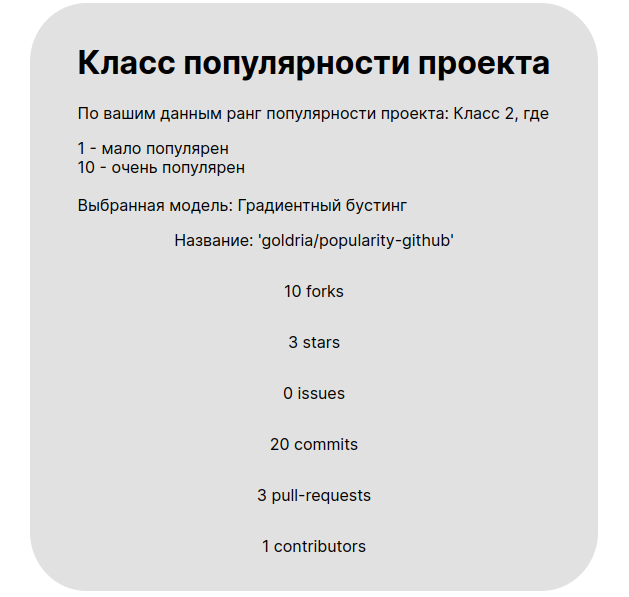
\includegraphics[scale=0.5]{pic/result-data.png}
        \caption{Форма для ввода данных}
        \label{ris:result-data}
    \end{figure}
\end{center}
\vspace{1.5em}
\newpage
\section{Тестирование}
\label{sec:Testings}
В данном разделе представлены результаты функционального тестирования и экспериментов по исследованию эффективности разработанной программы.
\subsection{Функциональное тестирование}

В ходе данного тестирования проверялось соответствие приложения
предъявленным функциональным требованиям. Тестирование приложения
проводилось вручную. В таблице~\ref{tab:тест} приведен протокол ручного тестирования основных аспектов работы системы.

\begin{table}[H]
    \setstretch{1.0}
    \caption{Функциональное тестирование приложения}
    \fontsize{12pt}{1em}\selectfont
    \vspace{1em}
    \begin{tabularx}{\linewidth}{|c|X|X|X|c|}
       \hline
        \textbf{№} & \textbf{Название теста} & \textbf{Действие} & \textbf{Ожидаемый результат} & \makecell{\textbf{Тест} \\ \textbf{пройден?}} \\ \hline
        1 & Проверка определения класса популярности. & На странице с вводом отправить данные и получить значение популярности. & Ранг популярности определен. & Да \\ \hline
        2 & Проверка прогнозирования звезд. & В форме на странице в вводом нажать на кнопку "Определить" и получить значение звезд. & Значение возможного количества звезд отображено.  & Да \\ \hline
        3 & Проверка ввода только численных значений. & На странице с вводом данных ввести значения, отличные от чисел. & В поля не вводятся нечисленные значения. & Да \\ \hline
        4 & Проверка отправки формы данных. & При незаполненных данных на странице ввода отправить форму. & Получено всплывающее уведомление, что поле не заполнено. & Да \\ \hline
        5 & Проверка выбора модели. & На главной странице выбрать "Модель регрессии" \ и отправить форму с выбранной моделью "Случайный лес". & На странице результатов отображены результаты после прогнозирования с помощью модели "Случайный лес". & Да \\ \hline
        \end{tabularx} 
    \label{tab:тест}
\end{table}
\vspace{2em}

\subsection{Вычислительные эксперименты}

\textbf{Оценка моделей классификации с помощью метрик}

Метрики представляют собой инструменты оценки эффективности алгоритмов классификации, позволяющие оценить качество предсказаний модели на основе различных аспектов ее работы~\cite{manning2008introduction}. В данном разделе рассматриваются основные метрики, широко применяемые в задачах классификации.

\textit{Матрица ошибок} (Confusion Matrix) -- это таблица, используемая для оценки производительности модели классификации, позволяющая визуализировать результаты предсказаний по каждому классу. Она представляет собой матрицу, когда реальные значения классов из тестового набора данных сравниваются с предсказанными моделью.\\

\begin{tabular}[]{|c|c|c|} 
\hline
    \multicolumn{1}{|c|}{} & \text{positive} & \text{negative} \\ \hline
    \text{positive} & \text{True Positive (TP)} & \text{False Positive (FP)} \\ \hline
    \text{negative} & \text{False Negative (FN)} & \text{True Negative (TN)} \\ \hline
\end{tabular} 
\\

В матрице ошибок присутствуют четыре основных термина: 

\begin{itemizecustom}
    \item True Positive (TP): Это количество объектов, которые модель верно предсказала как положительные (верно идентифицированные положительные классы).
    \item  True Negative (TN): Количество объектов, которые модель верно предсказала как отрицательные (верно идентифицированные отрицательные классы).
    \item  False Positive (FP): Также называется ошибкой первого рода. Это количество объектов, которые модель неверно предсказала как положительные, хотя они на самом деле относятся к отрицательному классу (ложноположительные результаты).
    \item  False Negative (FN): Также называется ошибкой второго рода. Это количество объектов, которые модель неверно предсказала как отрицательные, хотя они на самом деле относятся к положительному классу (ложноотрицательные результаты).
\end{itemizecustom}

Точность (Accuracy) представляет собой долю правильных предсказаний модели относительно общего числа предсказаний. Она вычисляется по формуле:

\[ Accuracy = \frac{TP + TN}{TP + TN + FP + FN} \]
\vspace{1.5em}

где \( TP \) - количество истинно положительных предсказаний, \( TN \) - количество истинно отрицательных предсказаний, \( FP \) - количество ложно положительных предсказаний и \( FN \) - количество ложно отрицательных предсказаний.

\textit{Точность класса} (Precision) измеряет долю истинно положительных предсказаний среди всех предсказанных положительных случаев, в то время как \textit{полнота класса} (Recall) измеряет долю истинно положительных предсказаний среди всех истинно положительных случаев. Они вычисляются по формулам:

\[ Precision = \frac{TP}{TP + FP} \]

\[ Recall = \frac{TP}{TP + FN} \]
\vspace{1.5em}

\textit{F-мера} (F1-score) представляет собой гармоническое среднее между точностью и полнотой класса и является компромиссом между ними. Она вычисляется по формуле:

\[ F1 = \frac{2 \cdot Precision \cdot Recall}{Precision + Recall} \]
\vspace{1.5em}

Для каждой из моделей была составлена матрица ошибок, отражающая, какое количество элементов модель смогла верно определить относительно того класса популярности проекта, к которому она была определена ранее. На рисунке~\ref{ris:class} представлена матрица ошибок Градиентного бустинга, который показал хороший результат в сравнении с другими моделями. Для остальных рассмотренных в работе моделей были составлены аналогичные матрицы ошибок. Результаты представлены в приложении Б. 

\begin{figure}[h]
    \centering
    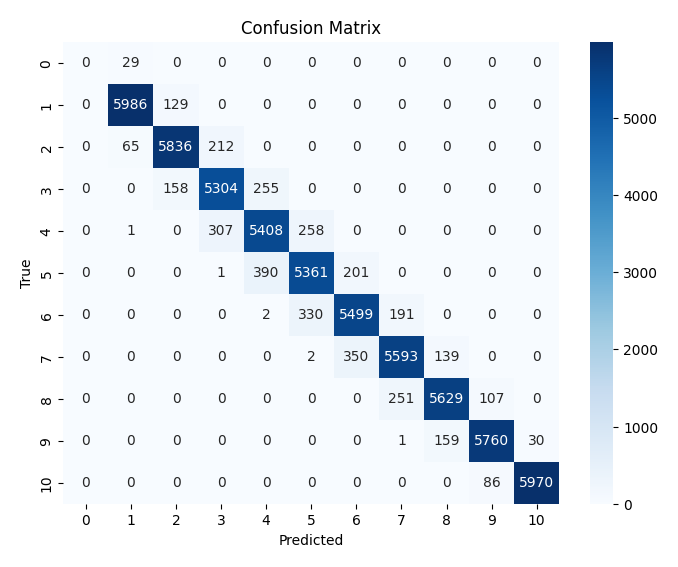
\includegraphics[width=0.9\linewidth]{pic/classification/gradient_boosting.png}
    \vspace{0.5em}\caption{Матрица ошибок Градиентного бустинга}
    \label{ris:class}
\end{figure}
\vspace{1em}

В рамках каждой модели есть свои параметры, которые влияют на обучение моделей, на точность определения проекта к классу популярности в зависимости от исходных параметров. Так, например, параметр n\_estimators указывает количество базовых моделей, которые будут объединены. Большее количество шагов может улучшить качество модели, но может увеличить время обучения. Значение random\_state управляет случайностью в модели. Задавая одно и то же значение, можно получить одинаковые результаты при каждом запуске обучения модели. В модели Градиентного бустинга есть параметр learning\_rate (float), который контролирует величину, на которую каждый базовый классификатор "учится" на ошибках предыдущих классификаторов.

Параметры помогают настроить модели таким образом, чтобы они давали оптимальные результаты для конкретного набора данных и задачи классификации. При этом изменение большинства параметров с целью улучшения точности ведет к значительному увеличению времени обучения модели. Время обучения тоже является важным критерием при выборе модели и параметров. 

В результате необходимо найти подходящее соотношение времени обучения и результатов метрик, для этого было проведено сравнение скорости обучения модели и результатов значений метрик на разных значениях параметра n\_estimators. На рисунке~\ref{ris:graph} представлен график зависимости времени обучения модели и результат значений метрик, где видно, что увеличение параметра начало всё меньше влиять на значения метрик, при этом время выполнения также растет, поэтому оптимально искать среднее значение. Для других моделей с хорошими показателями метрик были составлены аналогичные графики зависимостей. Результаты представлены в приложении В. 

\begin{figure}[h]
    \centering
    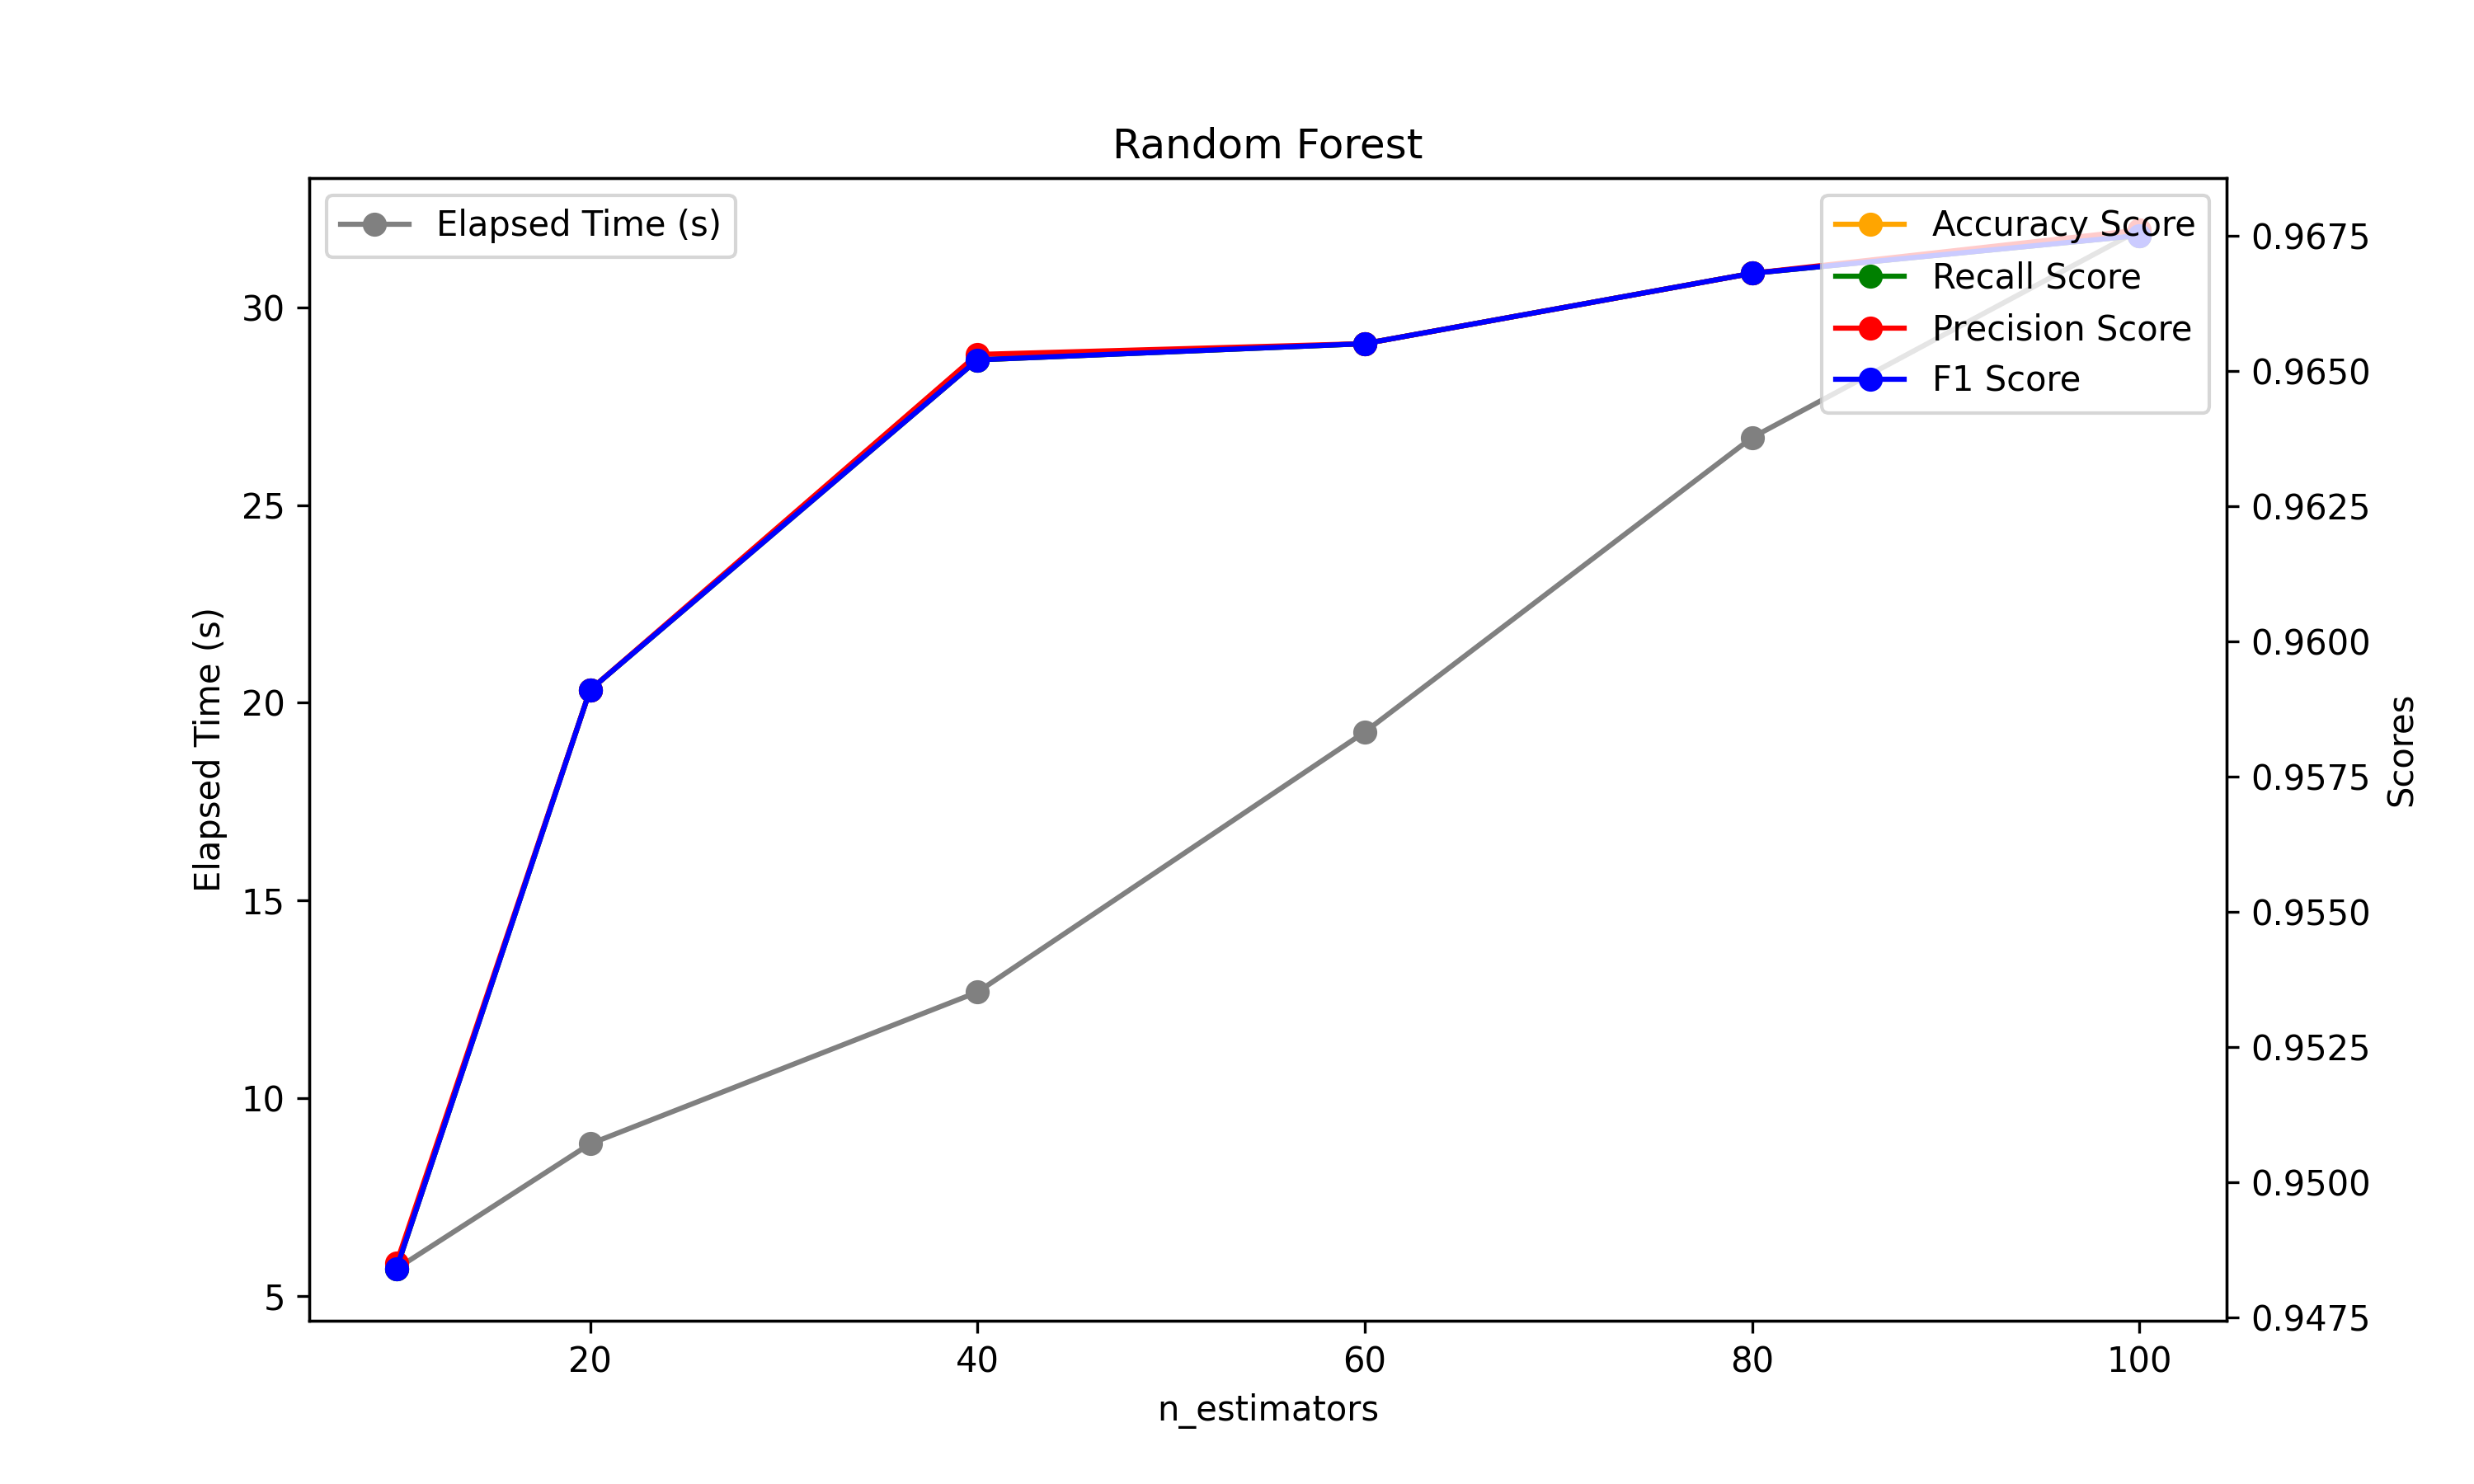
\includegraphics[width=1\linewidth]{pic/statistic/random_forest.png}
    \vspace{0.5em}\caption{График зависимости времени и метрик Случайного леса}
    \label{ris:graph}
\end{figure}
\vspace{1em}

После определения оптимальных значений в параметрах и оценке их времени выполнения в каждой модели было выполнено обучение и вычисление значений метрик. Результаты рассчитанных метрик для реализованных моделей классификации представлены в таблице~\ref{tabular:table-classification}. Чем ближе значение к 1, тем более точно модель способна определить класс.

\begin{table}[H]
    \onehalfspacing 
    \caption{Значения метрик моделей классификации}
    \medskip
        \begin{tabular}{|l|c|c|c|}
        \hline
        \backslashbox{}{}  & precision & recall & F-score \\ \hline
            Decision Tree & 0.9405 & 0.9406 & 0.9405 \\  \hline 
            Random Forest & 0.9675 & 0.9675 & 0.9675 \\  \hline 
            Gradient Boosting & 0.7463 & 0.7511 & 0.7689 \\  \hline 
            AdaBoosting & 0.3162 & 0.6698 & 0.2596 \\  \hline 
            Naive Bayes & 0.6258 & 0.6387 & 0.6273 \\  \hline 
        \end{tabular}
    \label{tabular:table-classification}
\end{table}
\vspace{1em}

\textbf{Оценка моделей регрессии с помощью метрик}

Метрики в задачах регрессии играют важную роль в оценке точности и эффективности модели. Они позволяют оценить, насколько хорошо модель соответствует реальным данным и насколько точны ее прогнозы. В данном разделе рассматриваются основные метрики, применяемые для оценки моделей регрессии.

\textit{Средняя абсолютная ошибка} (Mean Absolute Error, MAE) представляет собой среднее абсолютное значение разницы между фактическими значениями и прогнозируемыми значениями модели. Она вычисляется по формуле:

\[ MAE = \frac{1}{n} \sum_{i=1}^{n} |y_i - \hat{y}_i| \]
\vspace{0.5em}

где \( y_i \) - фактическое значение, \( \hat{y}_i \) - прогнозное значение, а \( n \) - количество наблюдений.
\vspace{1em}

\textit{Среднеквадратичная ошибка} (Mean Squared Error, MSE) измеряет среднеквадратичную разницу между фактическими значениями и прогнозируемыми значениями модели. Она вычисляется по формуле:

\[ MSE = \frac{1}{n} \sum_{i=1}^{n} (y_i - \hat{y}_i)^2 \]
\vspace{0.5em}

где \( y_i \) - фактическое значение, \( \hat{y}_i \) - прогнозное значение, а \( n \) - количество наблюдений.
\vspace{1em}

\textit{Коэффициент детерминации} (Coefficient of Determination, \( R^2 \)) измеряет пропорцию вариации зависимой переменной, объясненной моделью, к общей вариации зависимой переменной. Он принимает значения от 0 до 1 и чем ближе значение \( R^2 \) к 1, тем лучше модель соответствует данным. \( R^2 \) вычисляется по формуле:

\[ 
R^2 = 1 - \frac{\sum_{i=1}^{n} (y_i - \hat{y}_i)^2}{\sum_{i=1}^{n} (y_i - \bar{y})^2} 
\]
\vspace{0.5em}

где \( \bar{y} \) - среднее значение зависимой переменной. 

\vspace{1em}

Эти метрики предоставляют информацию о точности и качестве модели регрессии, помогая исследователям и практикам принимать информированные решения на основе результатов их работы.

Аналогично моделям классификации были определены оптимальные значения в параметрах. Результаты рассчитанных метрик для реализованных моделей регрессии представлены в таблице~\ref{tabular:table-regression}.

\begin{table}[H]
    \onehalfspacing \caption{Метрики задач регрессии}
    \medskip
        \begin{tabular}{|l|c|c|c|}
        \hline
            \backslashbox{}{}  & MSE & MAE & $R^2$ \\ \hline
            Decision Tree & 97601.26 & 466.59 & 0.2150 \\  \hline 
            Random Forest & 54962.27 & 355.25 & 0.5580 \\  \hline 
            Gradient Boosting & 55149.55 & 367.19 & 0.5563 \\  \hline 
            Linear Regression & 70683.04 & 530.50 &  0.4317 \\  \hline 
        \end{tabular}
    \label{tabular:table-regression}
\end{table}

Для оценки качества определения классов были сформированы отдельные тестовые наборы, наиболее наглядно отражающие принадлежность к рангам. Результаты представлены в приложении Г.
\newpage
\sectionnonumber{Заключение}
\label{sec:Conclusion}

В рамках данной работы была разработана система, осуществляющая подготовку данных, обучение моделей и определение класса популярности проектов в рамках GitHub.

При этом были решены следующие задачи.

\begin{enumerateparendot}
    \item Выполнен анализ предметной области и проведен обзор существующих решений.

    \item Выбран набор признаков и подготовлены данные по существующим репозиториям GitHub.

   \item Исследованы различные модели машинного обучения.

    \item Разработана система в виде веб-приложения, которая классифицирует проекты по популярности на основе выбранной модели.
\end{enumerateparendot}
\vspace{1em}

Дальнейшая работа будет направлена на рассмотрение разных критериев определения класса популярности и других параметров в рамках выборки набора данных для обучения.

\newpage
{\raggedright
\phantomsection\addcontentsline{toc}{section}{\refname}
\bibliographystyle{ugost2008}
\bibliography{thesis}
}
% \printbibliography[env=gostbibliography, sorting=ntvy]

\end{document}

% vim: set tw=72 syntax=tex:
